\documentclass {aldast}

\usepackage{makecell}
\usepackage{algorithm2e}

\documentType{Lecture Notes}
\documentNumber{1.2}
\title{Random Access Machines}
\author{F. Chauvel}


\begin{document}

\maketitle

\begin{abstract}
  We lay down some foundations: What are we trying to solve? What is
  an algorithm? What are data structures? How do they help? We also
  look at programs, pseudo-code and other techniques to describe
  algorithms. Finally we will look at one machine that can execute
  algorithms and see how it works and what it can and cannot do.
\end{abstract}


\section*{Introduction}
The main point of this course is to get better at solving programming
problems. We will do that by looking at many well-known problems and
their solutions. Practice makes perfect, there is no shortcut
here. This is particularly hard\sidenote{Algorithms and data
  structures form the basis of most programming competitions, and of
  some programming interviews}, but for now, let me explain what an
algorithm is.

\section{Computational Problems}

We are not solving any type of problems, but only \emph{computational
  problems}. So, what are these?  The official answer is: ``Problems
that one can solve with an algorithm''. Not very helpful at this point
since we have not yet defined an algorithm, but we will get there.

A computational problem associates an input to an output and specify
the properties that the output must satisfy. Both input and output are
``data'' that can be encoded as a sequence of 0 and 1. This includes
numbers, text, sound recordings, images, etc. Take the addition of two
natural numbers (i.e. integers) as an example. We can describe this
problem as the following mathematical function:

\begin{align}
  add: \mathbb{N} \times \mathbb{N} &\mapsto \mathbb{N} \nonumber \\
  add\, (x, y) & \mapsto x + y
\end{align}

Note that the '$+$' sign I used above does not tell us how to actually
carry out an addition. It simply denotes the ``addition'' concept and
I assume here that everyone will recognize it and know what it means
and implies (associativity, neutral element, etc.). If you already how
to add two natural numbers, then you know a solution (to solve this
problem), but we are looking only at the problem.

There are many types of computational problems. In \emph{decision
  problems} for example, the output is a Boolean value (yes or no),
such as testing whether a given number is a prime number. We will also
meet search problems, where we have to find a particular value in a
larger set, such as finding all the pairs of number whose sum is
10. Another type of problem is counting, where we try to figure out
the number of solutions to a another problem. Finally there is also
optimization problems, where we search for the solution that maximize
a specific criterion. All these problems can be described as
mathematical functions\sidenote{The concept of ``function'' exists
  both in programming and in mathematics, but means different
  things. Computational problems are described by mathematical
  functions.}.


\section{Algorithms}

How do we solve a problem? We need a procedure, that is a ``recipe''
that we can follow blindly---just like a machine---to get to the
result. These recipes or procedures are \emph{algorithms}:
Sequences of instructions that solve a computational problem.

\marginnote{
  \flushright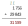
\includegraphics[width=3cm]{images/addition}
  \captionof{figure}{Adding two natural numbers}
  \label{fig:school-addition}
}[-1.5cm]

Returning to the addition of two natural numbers, we all have learned
in school an algorithm to do that. We take the two right-most digits,
we add them. If the result is greater than 10, we carry over a 1 onto
the next two digits on th left, and we repeat this until we have added
all pairs of digits. Figure~\ref{fig:school-addition} illustrates this
procedure.

\subsection{What Is an Algorithm?}

Unfortunately, I am not aware of a single formal definition, upon
which everyone agrees\sidenote{I found many attempts at a
  definition. See \cite{vardi2012,hill2016} or
  \href{https://en.wikipedia.org/wiki/Algorithm_characterizations}{algorithm
    characterizations} on Wikipedia for more details}. In this course,
I will reuse the definition given by D. Knuth in
TAOCP~\cite[p. 5--6]{knuth1978}, where he specifies the four following
properties:
\begin{itemize}
\item An algorithm has \emph{inputs and outputs}. It consume some data
  and produces some results. Our addition takes two natural numbers
  and produces their sum.
\item An algorithm is \emph{finite}: It must terminate at some point
  and cannot have an infinite number of steps. Our addition of two
  numbers stops when we have added all pairs of digits.
\item An algorithm is \emph{well-defined}, and each step is
  non-ambiguous. In our addition, each step is about reading, adding,
  comparing or writing numbers from 1 to 18.
\item An algorithm is \emph{effective} and can be carried out by
  either a machine or human with pen and paper. Children add numbers
  this way on a daily basis.
\end{itemize}



\paragraph{What about Data Structures?} To work efficiently, an
algorithm must organize its data carefully (inputs, outputs, and
intermediate results). Our addition example gives an nice example:
Children are told to align both numbers on their rightmost digit and
to place carryovers on top on the next number on the left. This is an
example of ``data structure'' per se.

\begin{takeaway}
  An \emph{algorithm} is a \emph{finite} sequence of
  \emph{non-ambiguous} instructions, which processes its inputs to
  produce the solution of a \emph{computational problem}. To work
  efficiently, algorithms store their data into dedicated \emph{data
    structures}.
\end{takeaway}

\subsection{How to Describe an Algorithm?}

I found several ways one can describe an algorithm: Natural language,
flowcharts, pseudo-code or programs.

\paragraph{Using Natural Language} The simplest way is to use plain
English, but this often lead to ambiguous text, which prevents
machines to follow our instructions. For example, we could describe
the addition of two number as follows:
\begin{enumerate}
\item Start with the pair of rightmost digits, which have not yet
    been added. If only one digit is available, assume 0 for the
    other.
  \item Add these two digits together with any carried over from
    previous step (if any) and mark down the result. If it is greater
    or equal to 10, subtract 10, mark down the difference, and carry
    over 1 onto the next end digit.
  \item If there are more digits on the left, return to Step 1.
\end{enumerate}

\paragraph{Using Flowcharts} Another human-friendly way is to use a
flowcharts, which visually portrays the sequence of
steps. Figure~\ref{fig:flowchart} shows a possible flowchart for the
addition of two natural numbers. The problem is that flowchart do not
really scale to complex algorithms.

\begin{figure}[htbp]
  \begin{center}
    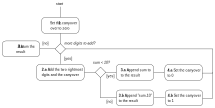
\includegraphics[width=\textwidth]{images/flowchart}
  \end{center}
  \caption{A flowchart depicting the addition of two natural numbers}
  \label{fig:flowchart}
\end{figure}

\paragraph{Using Pseudocode} A less space-demanding way is to use some
pseudo-code\sidenote{I will not use much pseudo code in this
  course. It is a matter of taste, but I found it very similar to
  writing high-level languages such as Python or Ruby, which one can
  run---for free.}. This resemble programming but does not refer to an
actual language. It just calls for a general understanding of
programming concepts. Regarding the addition of two numbers, we could
write something like:

\begin{algorithm}
  \KwData{$x,y \in \mathbb{N}^2$}
  \KwResult{$result = x + y$}
  $result \gets \emptyset$\;
  $length \gets \max(length(x), length(y))$\;
  $index \gets 1$\;
  $sum \gets 0$\;
  $carry \gets 0$\;
  \While{$index \leq length$ or $carry = 1$}{
    $sum \gets digit(x, index) + digit(y, index) + carry$\;
    \If{$sum > 9$}{
      $carry \gets 1$\;
      $sum \gets sum - 10$\;
    }
    $result \gets append(sum, result)$\;
    $index \gets index + 1$\;
  }
\end{algorithm}

\paragraph{Using a Program} If we do \emph{not} want to be ambiguous,
we can directly write a program using your favorite language. I
put below a Python program equivalent to the pseudo code
above\sidenote{Writing a program that adds two numbers this way is a
  complete nonsense. Addition is natively supported in all
  languages!}.

\inputminted{python}{code/sum.py}

\begin{takeaway}
  An algorithm is a pure abstract concept, which we cannot directly
  seize. It only surfaces when we describe it using a specific language
  or syntax.
\end{takeaway}

We still have a problem however. When we describe an algorithm, we
need to decide on \emph{basic actions} and we assume that
\emph{executor} (either a machine or a human) is able to perform
these. For example, to add two natural numbers, we have assumed the
existence of conditional statements, loops, arithmetic and logical
operations, etc. In the next section, we'll specify these actions using a
\emph{computation model}, which we will use throughout the remainder
of this course.

 
\section{Random Access Machines}

What do we expect from the ``agent'' that will execute our algorithms, be
it a human or a machine? Does it know arithmetic, logic? Maybe it can
only manipulate symbols? If we do not agree upon its capabilities, we
cannot describe, exchange or compare algorithms!

To this end, we will look at a minimal ``machine'' that can
nonetheless compute anything that is computable. This will clarify
what we can and cannot do. This machine, called \emph{random access
  machine} (RAM)~\cite{cook1973}, closely resembles an actual computer
with a CPU and a memory but is much simpler. Having this precisely
defined will turn out handy when we will look at correctness and
efficiency of algorithms.

\subsection{Architecture}

A random access machine (RAM) is a simplistic machine that mimics the
behavior of a real computer\sidenote{RAM is a \emph{computation
    model}: It defines what a computation can do. There are many
  others, such as Turing Machine, cellular automata, etc., but they
  are equivalent. We will come back to that in Lecture 12.2.}. It has
the three following components, as shown on Figure~\ref{fig:ram}.
\begin{itemize}
\item A central processing unit (CPU) that carries out arithmetic and
  logical operations. This CPU has two registers, namely \texttt{ACC}
  and \texttt{IP} which can both hold a single integer value.
  \begin{itemize}
  \item \texttt{ACC} is the \emph{accumulator} and holds
    intermediate results.
  \item \texttt{IP} is the \emph{instruction pointer}, and contains the
    address where the next instruction is located.
  \end{itemize}
\item A \emph{memory}, which can hold an infinity of integer
  values. Each memory cell has a unique address (also an integer)
  which enable reading and writing randomly throughout the memory.
\item An \emph{I/O device} that the machine uses to communicate with the
  user. We can think of this as a screen and a keyboard for example.
\end{itemize}

\begin{figure}[htbp]
  \begin{center}
    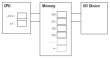
\includegraphics[width=0.8\textwidth]{images/ram}
  \end{center}
  \caption{The architecture of random access machines}
  \label{fig:ram}
\end{figure}

The RAM model remains a gross simplification. In a ``real''
computer, there dozens of registers, which can only contain a finite
amount of information (i.e, a number up to a limit). The same goes
for the memory, which is finite in practice, but includes various
level of caching. The principle are however the very same.

\subsection{Instructions}

The RAM instructions (i.e., the code of our programs) are stored in
the main memory, just like any other data. This is the core principle
behind the Von Neumann architecture: Code is just yet another type of
data.

\begin{table}[htbp]
  \begin{center}
    \begin{tabular}{r>{\ttfamily}lp{4cm}>{\ttfamily}p{3.5cm}}
      \toprule
      OP & Mnemonic & Description                                                                                                 & Semantic                          \\
      \midrule
      1  & LOAD n   & Load the value $n$ in the \texttt{ACC} register.                                                            & \makecell[tl]{ACC := n            \\IP := IP + 2 } \\[1cm]
      2  & ADD a    & Add the value contained at address $a$ to the \texttt{ACC} register.                                        & \makecell[tl]{ACC := ACC + Mem[a] \\ IP := IP + 2} \\[1cm]
      3  & SUB a    & Subtract the value contained at address $a$ from the \texttt{ACC} register.                                 & \makecell[tl]{ACC := ACC - Mem[a] \\ IP := IP + 2} \\[1cm]
      4  & STORE a  & Store the value of the \texttt{ACC} register in the memory at address $a$.                                  & \makecell[tl]{Mem[a] := ACC       \\ IP := IP + 2} \\[1cm]
      5  & JUMP a   & Reassign the \texttt{IP} register with the address $a$ only if the \texttt{ACC} register value is positive. & \makecell[tl]{if ACC >= 0         \\ ~~~IP := a \\ else \\ ~~~IP := IP + 2} \\[1.5cm]
      6  & READ a   & Read a value from the I/O device and store it at the given address $a$.                                     & \makecell[tl]{Mem[a] := I/O       \\ IP := IP + 2} \\[1cm]
      7  & PRINT a  & Print the value contained at the given address $a$ to the I/O device.                                       & \makecell[tl]{I/O := Mem[a]       \\ IP := IP + 2} \\[1cm]
      ?  & HALT -   & Stop the machine.                                                                                           & N/A                               \\
      \bottomrule
    \end{tabular}
  \end{center}
  \caption{The eight RAM instructions. \texttt{Mem[a]} denotes the
    value stored in memory at the address $a$. Note that \texttt{LOAD}
    takes a value whereas all other instructions accept an
    address. Any OP outside the range $[1, 7]$ stops the machine.}
  \label{tab:ram-instructions}
\end{table}

Table~\ref{tab:ram-instructions} details the eight instructions
available on RAM. Each instruction occupies two contiguous memory
cells: One for the operation code (OP), which indicates which
instruction must be executed, and one the operand. For example, two
contiguous memory cells with value 1 and 12 are interpreted as
\texttt{LOAD 12}, because 1 is the operation code of the \texttt{LOAD}
instruction and 12 is the operand. The machine would thus override the
value of the \texttt{ACC} register with the value 12, as explained in
Table~\ref{tab:ram-instructions}

\begin{takeaway}
  The RAM model defines the actions (i.e., the 8 instructions of
  Table~\ref{tab:ram-instructions}) that we can use to describe
  algorithms. This set is \emph{minimal}: Removing any action reduces
  the ``computational'' power of the machine.
\end{takeaway}

\paragraph{How does it work?} It reads two memory cells from the
address contained in the \texttt{IP} register. Then it executes this
instruction following the semantic given in
Table~\ref{tab:ram-instructions}, and start over. The machine stops
when it meets an unknown operation code.

\paragraph {Example: Adding two numbers}
Table~\ref{tab:ram-example} shows the complete memory layout of a tiny
program that reads two numbers and print their sum. The program stores
the numbers given by the user at addresses 50 and 51 respectively. It
also stores the sum at address 52.

\begin{table}[htbp]
  \begin{center}
    \begin{tabular}{>{\ttfamily}l>{\ttfamily}l>{\ttfamily}l}
      \toprule
      Addresses & Content & Interpretation \\
      \midrule
      00, 01 & 6, 50 & READ 50 \\
      02, 03 & 6, 51 & READ 51 \\
      04, 05 & 1,  0 & LOAD  0 \\
      06, 07 & 2, 50 & ADD  50 \\
      08, 09 & 2, 51 & ADD  51 \\
      10, 11 & 4, 52 & STORE 52 \\
      12, 13 & 7, 52 & PRINT 52 \\
      14, 15 & 0, 0 & HALT \\
      \bottomrule
    \end{tabular}
  \end{center}
  \caption{A sample program laid out in memory. The program reads two
    numbers through the I/O device and prints their sum back to the I/O
    device.}
  \label{tab:ram-example}
\end{table}

Given the memory shown by Table~\ref{tab:ram-example}, provided that
\texttt{IP} is initially set to 0, the RAM proceeds as follows:
\begin{enumerate}
\item The machine reads the memory cells at address 0 and 1 and
  interprets these as \texttt{READ 50}. It thus reads a value through
  the I/O device and stores it at the given address (i.e., 50). It
  then increments \texttt{IP} by 2, which now contains the value 2.
\item With \texttt{IP} holding 2, the machine reads addresses 2 and
  3, which it interprets as \texttt{READ 51}. It thus reads another
  value through the I/O device, stores it at address 51, and then
  increments \texttt{IP} by 2 again.
\item With \texttt{IP} being now 4, the machine reads addresses 4 and
  5, which it interprets as \texttt{LOAD 0}. It thus sets the
  \texttt{ACC} register to 0, and then increments \texttt{IP} by 2.
\item \texttt{IP} now equals 6, The machine reads addresses 6 and
  7, which it interprets as \texttt{ADD 50}. It thus adds the value at
  address 50 to the \texttt{ACC} and then increments \texttt{IP} by 2.
\item \texttt{IP} now contains 8. The machine reads addresses 8 and 9,
  which it interprets as \texttt{ADD 51}. It thus adds the value
  stored at address 51 to the \texttt{ACC} register and then increase
  IP by 2.
\item \texttt{IP} is now 10 and the machine reads addresses 10 and 11,
  which it interprets as \texttt{STORE 52}. It writes the value
  contained in the \texttt{ACC} register into the memory at address
  52. It then increments \texttt{IP} by 2, which now holds 12.
\item It now reads addresses 12 and 13, and interprets it as
  \texttt{PRINT 52}. The machine thus sends the value stored at
  address 52 to the I/O devices. It then increments \texttt{IP} by 2.
\item The next instruction, starting at address 14 stops the machine.
\end{enumerate}

At this low level, we see clearly the instructions carried out by the
machine, their meaning and their order. Writing such ``machine code''
is however not the most effective way to write programs. In real life,
we use compilers (or interpreters) that generate machine code from
higher-level programs like C/C++, Java, Python or LISP to name only a
few. These languages rely on three key constructs\sidenote{At least
  for imperative languages such as C, Java, Pascal, BASIC, etc.}:
variable assignments, conditional statements, and loops. We will touch
upon the translation from high-level language to machine code in
Lecture 2.1.

Despite its simplicity, the RAM model is \emph{as powerful as a real
  machine}. Anything that can be computed on a real machine can be
computed on RAM, it is just extremely slow. The RAM model is complete
and minimal: It contains everything (assignment, loops, and
conditions) but nothing can be removed without decreasing its
``computation'' power.

\section*{Conclusion}
We now know the difference (and the relationships) between a problem,
an algorithm and a program. We also know how a machine can store and
execute algorithms using programs written in machine code. Next, we
will see how one can establish the correctness of an algorithm:
Providing evidences that an algorithm actually solves a given problem.


\bibliographystyle{acm}
\bibliography{references}

\end{document}